%! Author = Philipp Emmenegger
%! Date = 08/06/2021

\section{Backlog Management}
\subsection{User Stories}
\begin{itemize}
    \item Informal description from the perspective of a user
    \item May be written by anyone
\end{itemize}

\subsection{Tasks}
\begin{itemize}
    \item Work items
    \item Created as part of the Sprint Planning / Refinement meeting
    \item Be specific
    \item Should be small
    \item Assign categories
    \item Use a workflow
    \item Track real efforts
\end{itemize}

\subsection{Epics}
\begin{itemize}
    \item Rough description of something that might be needed in the future
    \item Same format as User Stories, omit details not yet needed
\end{itemize}

\subsection{Refinement Meeting}
\begin{itemize}
    \item Refine the product backlog with the whole scrum team
    \item Keep the backlog in a good shape
    \item No official Scrum event
\end{itemize}

\subsection{Story Maps}
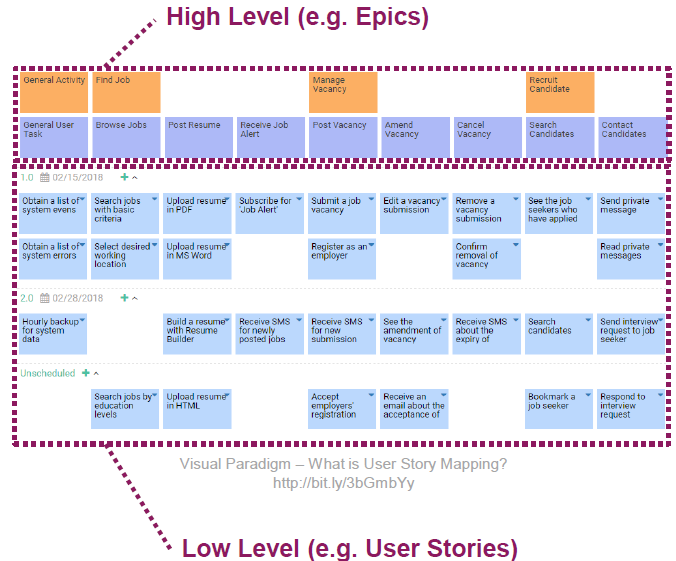
\includegraphics[width=\linewidth]{../img/story_maps.png}
\begin{itemize}
    \item Sort by activity horizontally
    \item Sort by priority vertically
    \item Usefull for release planning (MVP functionality)
    \item Can be used to create an initial backlog
\end{itemize}

\subsection{Release Planning}
\textbf{Requirements}
\begin{itemize}
    \item Estimates for all required functionality
    \item Velocity of the team
\end{itemize}
\textbf{Estimates}
\begin{itemize}
    \item Can be made in Refinements
\end{itemize}
\textbf{Velocity}
\begin{itemize}
    \item best measured in iterations
    \item can only be measured after executing some iterations
    \item otherwise use estimates / historical data
    \item update it regularly
\end{itemize}

\subsection{Prioritization}
\subsubsection{MVP approach}
\begin{itemize}
    \item All features mandatory for the MVP have the highest prio
    \item Extendable to multiple releases
\end{itemize}
\subsubsection{Other Factors}
\begin{itemize}
    \item Task of the Product Owner to choose the right factors
    \item Financial value
    \item Cost of developing
    \item New knowledge
    \item Amount of risk
    \item Desirability
\end{itemize}

\subsubsection{Kano Model}
\textbf{Threshold Attributes}
\begin{itemize}
    \item Basic features that customers expect
    \item Having a lot increases satisfaction only slightly
\end{itemize}
\textbf{Performance Attributes}
\begin{itemize}
    \item Not necessary, but welcome
    \item Linear increases in customer satisfaction
\end{itemize}
\textbf{Excitement Attributes}
\begin{itemize}
    \item Surprises the customer
    \item Huge impact on customer satisfaction
\end{itemize}

\subsubsection{MoSCoW Method}
\textbf{Must have}
\begin{itemize}
    \item Critical to the current delivery timebox
\end{itemize}
\textbf{Should have}
\begin{itemize}
    \item Important, but not necessary
\end{itemize}
\textbf{Could have}
\begin{itemize}
    \item Desirable, but lower prio
\end{itemize}
\textbf{Won't have}
\begin{itemize}
    \item Not planned into this delivery timebox
\end{itemize}

\subsubsection{The Big Wall}
\begin{itemize}
    \item Used to prioritize a big backlog
    \item \textbf{Step 1:} Devs sort all items horizontally by their relative size
    \item \textbf{Step 2:} Business owners vertically sort all items by prio
\end{itemize}

\subsection{Estimation}
\textbf{Why is it hard?}
\begin{itemize}
    \item You must estimate something you never built before
    \item Requirements change
    \item Devs focus on coding - forget the rest
    \item Developed by teams - individuals have different qualities
    \item Investing more time into estimation will \textbf{not} increase the accuracy
\end{itemize}

\subsubsection{Agile Estimation}
\begin{itemize}
    \item Estimate on different levels
    \begin{itemize}
        \item \textbf{Rough estimates} - used for Epics
        \item \textbf{Improved estimates} - used for User Stories
        \item \textbf{Elaborate estimates} - used for tasks
    \end{itemize}
    \item Improved estimates based on feedback cycles
    \item Given by the people that perform the task
    \item Done by the whole team
\end{itemize}

\textbf{Absolute and Relative}
\begin{itemize}
    \item Easier to estimate relative
    \item Based on actual feedback / velocity
\end{itemize}

\textbf{Units}
\begin{itemize}
    \item Hours
    \item T-Shirt sizes
    \item etc.
\end{itemize}

\textbf{Scales}
\begin{itemize}
    \item Too many options
    \item Predifined set for estimation
    \item Commonly used scales:
    \begin{itemize}
        \item Normal: 1,2,3,5,8,13,20,40, ...
        \item Fibonacci: 1,2,3,5,8,13,21,34, ...
        \item etc.
    \end{itemize}
\end{itemize}

\textbf{Planning Poker}
\begin{itemize}
    \item Avoids influence of other participants
    \item Emphasizes discussions about requirements
    \item Good tool-support available
\end{itemize}









